\placelogofalse
\begin{frame}{waLBerla}
\begin{columns}
\column{0.48\linewidth}
\begin{outline}
  \1 waLBerla framework 
  \2 Introduced in \cite{Bauer2021} (2021)
  \2 HPC-scale simulations
  \2 Stencil problems specifically
  \2 Bring your Compute Kernels
  \1 Provides:
  \2 Multi-node domain partitioning
  \2 Communication patterns 
  \2 Checkpoints
\end{outline}
\column{0.48\linewidth}
\begin{center}
  \shadowimage[width=0.8\linewidth]{juwels.png}
  \vspace{0.5cm}
  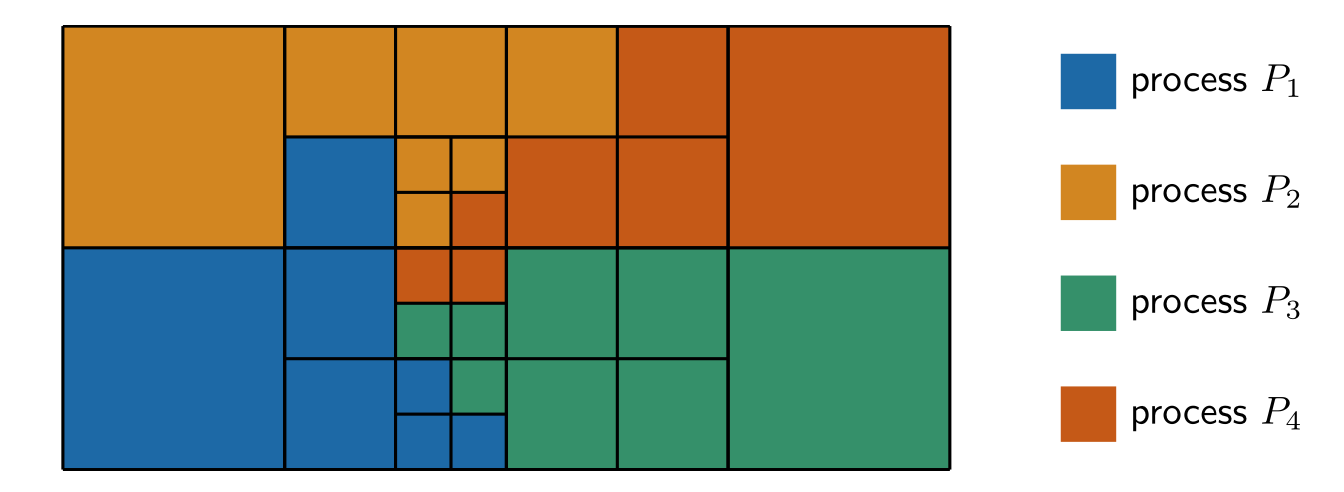
\includegraphics[width=0.8\linewidth]{walberla_partition.png}
  \vspace{0.5cm}
  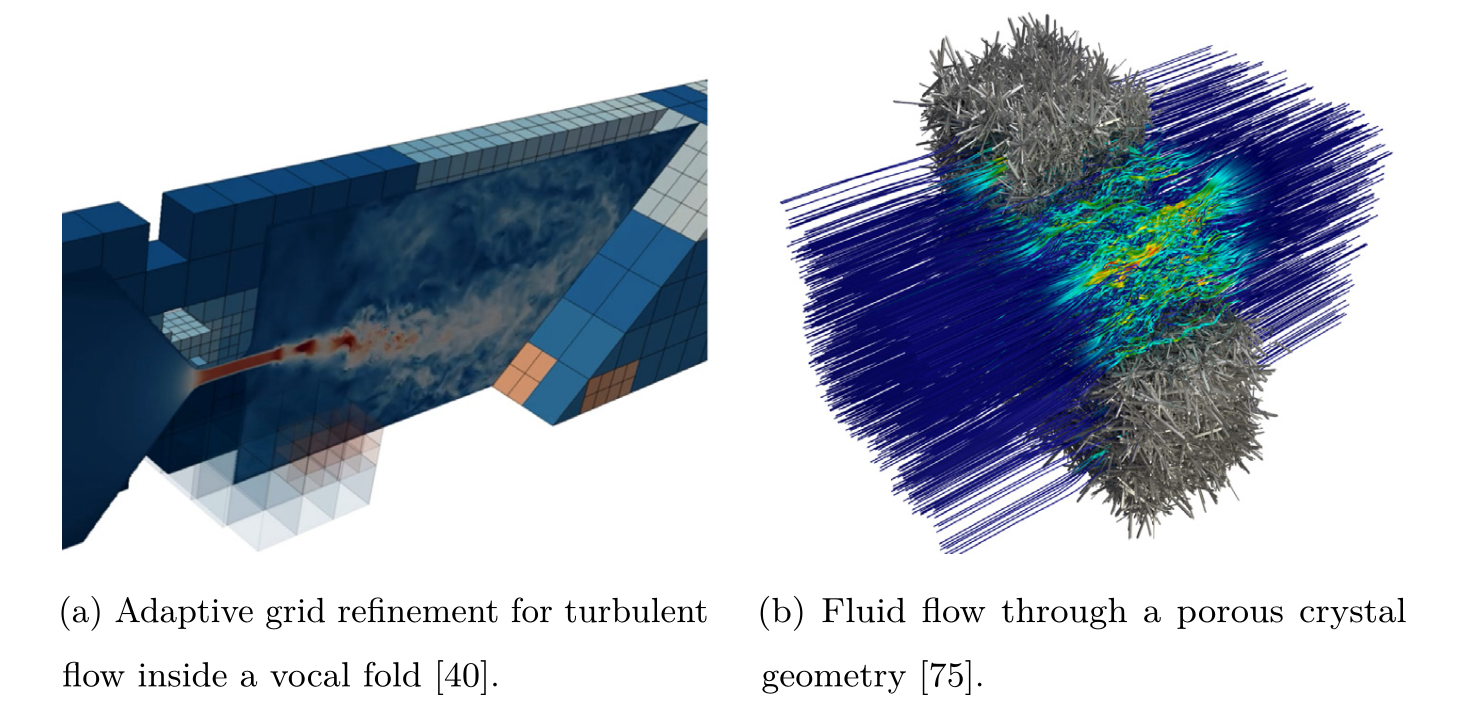
\includegraphics[width=0.8\linewidth]{walberla_examples.png}
\end{center} 
\end{columns}
\blfootnote{From \href{t}{TODO}, \cite{Bauer2021}}
\end{frame}
\placelogotrue

